%
% File eamt18.tex
%
% Contact: cettolo@fbk.eu, mlf@dlsi.ua.es

%%% To ease future customizations, various replaceables have been paramaterized
%%% as listed in the newcommands section

\documentclass{flammie}
%\usepackage{mtsummit2019}
%\usepackage{times}
\usepackage{url}
\usepackage{latexsym}
\usepackage[small,bf]{caption} % added MLF 20171211
%\setlength\titlebox{6.5cm}    % Expanding the titlebox
%%% YOUR PACKAGES BELOW THIS LINE %%%

\usepackage[inline]{enumitem}
\usepackage{booktabs}

\newif\iffinal%
\finaltrue%

\newcommand{\confname}{MT Summit 2019}
\newcommand{\website}{https://www.mtsummit2019.com}
\newcommand{\urlwebsite}{https://www.mtsummit2019.com}
\newcommand{\contactname}{the general chair, Andy Way}
\newcommand{\contactemail}{\texttt{andy.way@adaptcentre.ie}}
\newcommand{\conffilename}{mtsummit2019}
\newcommand{\downloadsite}{https://www.mtsummit2019.com/submissions}
\newcommand{\paperlength}{$9$ (nine)~}
\newcommand{\shortpaperlength}{$6$ (six)~}
\newcommand{\projectlength}{$1$ (one)~}
\newcommand{\translatorlength}{$1$ (one)~}

\title{Workflows for kickstarting RBMT in virtually No-Resource Situation}

\iffinal%
\author{Tommi A Pirinen\
  Universität Hamburg,\\
  Hamburger Zentrum für Sprachkorpora\\
  Max-Brauer-Allee 60, Hamburg\\
  {\tt tommi.antero.pirinen@uni-hamburg.de}}
\fi

\date{}

\begin{document}
\maketitle
\begin{abstract}
    In this article we describe a work-in-progress best learnt practices on how
    to start working on rule-based machine translation when working with
    language that has virtually no pre-existing digital resources for NLP use.
    We use Karelian language as a case study, in the beginning of our project
    there were no publically available corpora, parallel or monolingual
    analysed, no analysers and no translation tools or language models. We show
    workflows that we have find useful to curate and develop necessary NLP
    resources for the language. Our workflow is aimed also for no-resources
    working in a sense of no funding and scarce access to native informants, we
    show that building core NLP resources in parallel can alleviate the problems
    therein.
\end{abstract}

\section{Introduction}

A lot of research goes into working with low-resource situation, however, in 
context of large international conferences today, loww-resources can mean
anything from having millions and millions of lines of parallel
corpus\footnote{\url{http://www.statmt.org/wmt19/parallel-corpus-filtering.html}}
to ``anything except English''. For this work we consider the lowest-resourced
languages in the group of languages we work with, namely those having virtually
no widely known publicly accessible or available resources at the start of our
project, and for which we aim to search, curate and create the necessary
resources. This is a work-in-progress, but we believe we have already gathered
enough promising results to give some \textit{best recommended practices} on
how to start working on a language seemingly lacking all \textit{natural
language processing} (NLP) resources.

For the machine translation part we are working on doing a \textit{rule-based
machine translation} (RBMT) and specifically one between a minority language
(Karelian) and a closely related more-resourced language (Finnish), in the first
phase. The translator is bidirectional, i.e.\ we translate both Finnish to
Karelian and vice versa.  The work for majority language machine translations
(e.g.\ English and Russian) is reserved for the future after some resources have
been built.  We have chosen this for a number of reasons, firstly the task is
much easier when working with a related language than a typologically unrelated
one, and secondly there is a body of good results using RBMT of closely related
in further resource building, for example for Spanish-related languages in the
Wikipedia content translation.

The article is organised as follows, first in Section~\ref{sec:background} we
describe the background and rationale for this project, in
Section~\ref{sec:workflow} we describe our approach and methodology for RBMT
building, in Section~\ref{sec:results} we describe our results so far and
finally in the Section~\ref{sec:conclusion} we discuss findings and lay out
future work.

\section{Background}\label{sec:background}

One of the problems, we have identified in the past in building NLP resources
for minority languages, is that same or similar work ends up doing multiple
times between different scholars, or even within a single project of same
minority language. This is not very ideal situation, when resources like native
informants or skilled scholars are scarce. A typical example might be that a
documentary linguistics effort builds a corpus of annotated texts, that
includes hand annotated linguistic analysis, glosses and translations, while
computational linguists build a morphological analyser, treebank and machine
translator by hand from scratch as well. What we aim to achieve is synergy
between these two different research practices.

The technological methodology used in this project is based on following:
\begin{itemize}
    \item The rule-based machine translation is provided by
        apertium~\cite{apertium}.
    \item The morphological analyser-generator is based on the HFST
        engine~\cite{linden2009hfst}
    \item The morphological disambiguation is based on Constraint
        Grammar~\cite{karlsson1990constraint}
    \item annotation format is based on Universal dependencies~\cite{ud24}
\end{itemize}

This article describes what is still a work-in-progress, at this stage we are
evaluating how the approach is and if we should make a project in building the
supporting software for the methodology and language resource building. That is
to say we have the workflows in place and the supporting software is built as we
proceed with the project.
Some of the workflows described here have been previously tested in building
larger well-resourced machine translators, for example in~\cite{pirinen2018rulebased}.
Based on experiences of this project, we could estimate that the effort needed
is around 20,000 lines annotated and translated to get a comparable results as
out of the box neural system~\cite{pirinen2019neural}, this is however a
result achieved on two unrelated languages both of which aren't English, so
results on related non-English languages may be different.

We have selected to use a rule-based approach to machine-translation for this
project. Since rule-based approaches have somewhat fallen out of popularity in
recent years, it needs strong arguments to select this approach in favour of
others. For this purpose we have a check-list for which languages are to be used
with which approaches first:

\begin{itemize}
    \item Closely related languages: Finnish and Karelian are very closely
        related languages
    \item Lack of Parallel resources: Karelian has virtually zero
        digital resources
    \item Existence of written grammars: We have number of grammars to
        help~\cite{zaikov2013vienankarjalan}
\end{itemize}

One of the reasons we started to develop an approach to language resource
creation that can produce multiple language resources fast, is that we have
prior experience in \begin{enumerate*}
    \item building computational linguistic resources like
morphological analysers from the scratch without considering the corpus creation
or documentary linguistics and
    \item building language documentation corpora from
        the scratch without considering creation of dictionaries.
\end{enumerate*}
The ideal result of this project is to develop a method that empowers
computational linguists to work on their preferred form of language
documentation and corpus creation and makes use of the expert work put in. This
can always be achieved afterhands by scraping the produced corpora or data, but
our plan is to introduce that as a part of workflow.

For other projects that have aimed to achieve similar goals, many are related
to other rule-based machine translation efforts within the free/open source
rule-based machine translation community, e.g.\cite{washington2014finite}.
On larger scale in the NLP community there have been several attempts to
make computational linguists and documentary linguists work together towards
common goal in this manner, for
example~\cite{maxwell2008joint,blokland2015language}

The basis of this RBMT system between Karelian and Finnish is that we also have
a large coverage stable Finnish system already available~\cite{omorfi}.
Karelian on the other hand has no resources, and is described by the ethnologuy
as threatened\footnote{\url{https://www.ethnologue.com/language/krl}}.  We
could have also tested an unrelated language with large coverage dictionary,
for example Russian-Karelian  would be useful for the target audience, or build
a machine translation between two under-resourced closely related languages,
like Karelian and Livvi, which is a closely related language with slightly
more resources than Karelian but much less than Finnish.

Finally, for social and political reasons, there is a growing interest in
Karelian language and culture, and while there is a number of projects on
the linguistic aspects and language learning, there is a lack of
language technology-based projects in the field. Our aim is to fill that
hole.


\subsection{Languages}

The language we use a case study is Karelian, a minority Uralic language spoken
mainly in Republic of Karelia in Russia and in Finland. It is closely related
to Finnish, Livvi and Ludic, but they are not mutually intelligible for an
individual without at least some linguistic training. The naming of different
languages and varieties related to Karelian is often confusing, what we aim to
describe here is in line of ISO 639--3 language code \textit{krl}; see the
number 1 in the map in
Figure~\ref{fig:krl-map}\footnote{\url{https://commons.wikimedia.org/wiki/File:Map_of_Karelian_dialects.png}}
for the geographic distribution. For the machine translation task, in first
phase we build a Karelian---Finnish translator.

\begin{figure}
    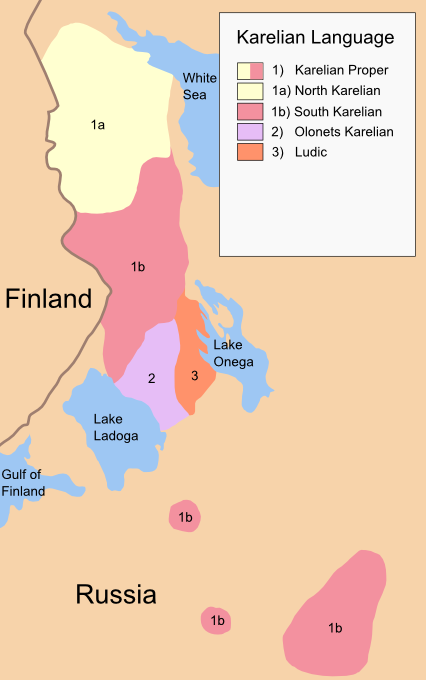
\includegraphics[width=0.48\textwidth]{Map_of_Karelian_dialects.png}
    \caption{Map of Karelian languages, the number 1 is Karelian that
    we study in this article, numbers 2 and 3 are closely related languages
    that are in some literature refered to as Karelian as well, but are
    separate languages and do not belong under the krl language code in
    ISO standard.\label{fig:krl-map}}
\end{figure}

\section{Workflow}\label{sec:workflow}

The workflow that we have reached at this point of the project is a synthesis
of traditional workflow in documentary linguistics and workflows in building
corpora and analyser writing, specifically in traditional rule-based systems.
In documentational linguistics we have drawn experience and inspiration from
\textit{SIL Fieldworks Explorer} (FLeX) and the rule-based workflows are
loosely based in tradition of Finite State Morphology.

The first part of the workflow is acquiring corpora, which for unresourced
minority is relatively difficult task, at the beginning of our project we aimed
to use web-as-corpus approach. During categorising the downloaded data
into languages we found also a corpus repository with a free to use open source
compatible licencing
policy\footnote{\url{http://dictorpus.krc.karelia.ru/en/corpus/text}}, which on
top of expert made language classification has the advantage that we can keep
full documents instead of shuffled sentences.


The actual corpus building workflow consists of two parts that can be
alternated between, annotation and lexicon building. With annotation, we can
work on any of the following tasks: lemmatising and pos tagging, morphological
analysis, syntactic treebanking and machine translation. On the other side
lexicon building we build the morphological lexicon for a finite-state analyser,
and a bilingual lexicon for rule-based machine translation. A UML-style
graph of the process is shown in figure~\ref{fig:translation}.

\begin{figure}
    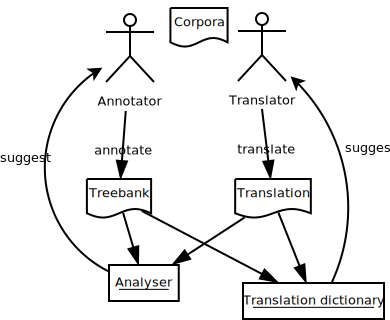
\includegraphics[width=0.48\textwidth]{process-uml}
    \caption{A UML-style chart of the annotation and translation
    process\label{fig:translation}}
\end{figure}

The main contribution of this workflow is that both of the tasks feed into
the other task, that is annotated corpora can be immediately used for entry
generation of the lexicons, and the analysers and machine translators
built from the lexicons are used to generate n-best lists from which annotators
can choose the annotations.

We provide a real world example here: An annotator starts working on a new
document that contains sentences: ``Pelih ošallistu 13 henkie'' (13 people
participated in the play) the annotator annotates in UD format:
\begin{scriptsize}
\begin{verbatim}
1 peliin peli  NOUN  Number=Sing|Case=Ill 2 obl _ _
2 ošallistu ošallistuo VERB  Number=Sing|Tense=Pres 0 root _ _
3 13 13 NUM Number=Sing|NumType=Card 4 nummod _ _
4 henkie henki NOUN  Number=Sing|Case=Par 2 nsubj _ _
\end{verbatim}
\end{scriptsize}
and provides Finnish translation like ``Peliin
osallistui 13 henkilöä''.  The annotation is used to generate entries for
monolingual dictionary of Karelian, i.e. \verb|peli<n>|,
\verb|ošallistuo<vblex>|, \verb|13<num>|, and \verb|henki<n>|, the lexicon
writer can simply fill in the necessary informations to inflect the words
properly. The entries can likewise be generated to bilingual dictionary, if 1:1
translation match to existing target language analyses is trivial, we get
\verb|peli<n>:peli<n>| etc.\ among the suggested entries. Now, when the
annotator gets back to annotating and translating the next sentences of the
document and runs into: ``Pelissä ”tapettih” šamoin Ilmarini'' (Ilmarinen was
also killed in the game), the first token ``Pelissä'' has suggested annotation
\texttt{peli NOUN Number=Sing|Case=Ine} as well as suggested translation.


\section{Results}\label{sec:results}

In a short time we have managed to build a rule-based machine translation
system. We detail the system in Table~\ref{table:sizes}. The corpus built
so far in this proto-typing phase of the project has been built by one
expert annotator, working on spare time for three months in other words in
only handful of work hours.

At the current moment we do not have enough bilingual corpora to measure the
translation quality yet but we hope to include a BLEU and WER evaluations of
the translation quality by the time we submit a camera-ready version of the
paper.

\begin{table}
    \begin{tabular}{lrr}
        \toprule
         & Tokens & Sentences \\
        \midrule
        Annotations & 3094 & 228 \\
        Translations & 1144 & 161 \\
        \bottomrule
    \end{tabular}
    \caption{The size of Karelian---Finnish corpus at the time of
    writing.\label{table:sizes}}
\end{table}

The corpora will be released on github via the Apertium project for the
translations and possibly also disambiguated corpora, and via Universal
dependencies project for the annotated corpus. Both retain the CC BY
licence of the original raw text data. The dictionaries and analysers
are also released via the Apertium using the GNU General Public Licence.

\section{Concluding remarks}\label{sec:conclusion}

We have found that we can rapidly build a solid base of natural language
resourcses suitable for rule-based machine translation and we aim to extend the
approach to more Uralic languages in near future. Furthermore the approach
prototyped in this paper has been found very motivating and nice to work with
in the future we will look at building a more approachable graphical user
interface for it.

The approach we describe here is especially suitable in no-resources starting
situation, even a limited amount of resources will open more workflows, more
technical possibilities to aid in the initial part of the corpus building and
resource building. However, we still think this approach may be useful as a
part of balanced corpus building approach in a research project for any lesser
researched language.

One of the things that we are looking forward to is to test the advances in
neural methods in very low resource
situation,~\cite{neubig2018rapid}\footnote{We thank the anonymous reviewers for
bringing this line of work to our attention }this would be particularly suitable
for Karelian-to-Finnish direction as Finnish is well-resourced.

\bibliographystyle{mtsummit2019}
\bibliography{loresmt2019}


\end{document}
